\documentclass[twoside]{book}

% Packages required by doxygen
\usepackage{fixltx2e}
\usepackage{calc}
\usepackage{doxygen}
\usepackage[export]{adjustbox} % also loads graphicx
\usepackage{graphicx}
\usepackage[utf8]{inputenc}
\usepackage{makeidx}
\usepackage{multicol}
\usepackage{multirow}
\PassOptionsToPackage{warn}{textcomp}
\usepackage{textcomp}
\usepackage[nointegrals]{wasysym}
\usepackage[table]{xcolor}

% NLS support packages
\usepackage[spanish]{babel}
% Font selection
\usepackage[T1]{fontenc}
\usepackage[scaled=.90]{helvet}
\usepackage{courier}
\usepackage{amssymb}
\usepackage{sectsty}
\renewcommand{\familydefault}{\sfdefault}
\allsectionsfont{%
  \fontseries{bc}\selectfont%
  \color{darkgray}%
}
\renewcommand{\DoxyLabelFont}{%
  \fontseries{bc}\selectfont%
  \color{darkgray}%
}
\newcommand{\+}{\discretionary{\mbox{\scriptsize$\hookleftarrow$}}{}{}}

% Page & text layout
\usepackage{geometry}
\geometry{%
  a4paper,%
  top=2.5cm,%
  bottom=2.5cm,%
  left=2.5cm,%
  right=2.5cm%
}
\tolerance=750
\hfuzz=15pt
\hbadness=750
\setlength{\emergencystretch}{15pt}
\setlength{\parindent}{0cm}
\setlength{\parskip}{3ex plus 2ex minus 2ex}
\makeatletter
\renewcommand{\paragraph}{%
  \@startsection{paragraph}{4}{0ex}{-1.0ex}{1.0ex}{%
    \normalfont\normalsize\bfseries\SS@parafont%
  }%
}
\renewcommand{\subparagraph}{%
  \@startsection{subparagraph}{5}{0ex}{-1.0ex}{1.0ex}{%
    \normalfont\normalsize\bfseries\SS@subparafont%
  }%
}
\makeatother

% Headers & footers
\usepackage{fancyhdr}
\pagestyle{fancyplain}
\fancyhead[LE]{\fancyplain{}{\bfseries\thepage}}
\fancyhead[CE]{\fancyplain{}{}}
\fancyhead[RE]{\fancyplain{}{\bfseries\leftmark}}
\fancyhead[LO]{\fancyplain{}{\bfseries\rightmark}}
\fancyhead[CO]{\fancyplain{}{}}
\fancyhead[RO]{\fancyplain{}{\bfseries\thepage}}
\fancyfoot[LE]{\fancyplain{}{}}
\fancyfoot[CE]{\fancyplain{}{}}
\fancyfoot[RE]{\fancyplain{}{\bfseries\scriptsize Generado por Doxygen }}
\fancyfoot[LO]{\fancyplain{}{\bfseries\scriptsize Generado por Doxygen }}
\fancyfoot[CO]{\fancyplain{}{}}
\fancyfoot[RO]{\fancyplain{}{}}
\renewcommand{\footrulewidth}{0.4pt}
\renewcommand{\chaptermark}[1]{%
  \markboth{#1}{}%
}
\renewcommand{\sectionmark}[1]{%
  \markright{\thesection\ #1}%
}

% Indices & bibliography
\usepackage{natbib}
\usepackage[titles]{tocloft}
\setcounter{tocdepth}{3}
\setcounter{secnumdepth}{5}
\makeindex

% Hyperlinks (required, but should be loaded last)
\usepackage{ifpdf}
\ifpdf
  \usepackage[pdftex,pagebackref=true]{hyperref}
\else
  \usepackage[ps2pdf,pagebackref=true]{hyperref}
\fi
\hypersetup{%
  colorlinks=true,%
  linkcolor=blue,%
  citecolor=blue,%
  unicode%
}

% Custom commands
\newcommand{\clearemptydoublepage}{%
  \newpage{\pagestyle{empty}\cleardoublepage}%
}

\usepackage{caption}
\captionsetup{labelsep=space,justification=centering,font={bf},singlelinecheck=off,skip=4pt,position=top}

%===== C O N T E N T S =====

\begin{document}

% Titlepage & ToC
\hypersetup{pageanchor=false,
             bookmarksnumbered=true,
             pdfencoding=unicode
            }
\pagenumbering{roman}
\begin{titlepage}
\vspace*{7cm}
\begin{center}%
{\Large Redes de Comunicaciones II \\[1ex]\large 1.\+0 }\\
\vspace*{1cm}
{\large Generado por Doxygen 1.8.11}\\
\end{center}
\end{titlepage}
\clearemptydoublepage
\tableofcontents
\clearemptydoublepage
\pagenumbering{arabic}
\hypersetup{pageanchor=true}

%--- Begin generated contents ---
\chapter{P3-\/ Seguridad S\+SL}
\label{index}\hypertarget{index}{}En esta página se encuentra disponible la documentación de librería S\+SL de la práctica 3 de Redes de Comunicaciones II, grupo 2313, pareja 6.

\section*{Librería S\+SL}

La librería S\+SL proporciona una capa superior a las funciones de los servidores echo proporcionados para la práctica. En ella se encuentran las funciones de fijación, conexión, envío y recepción mediante la capa S\+SL de socket. 
\begin{DoxyItemize}
\item \hyperlink{inicializar_nivel_SSL}{Inicialización de S\+SL} 
\item \hyperlink{fijar_contexto_SSL}{Fijación del contexto S\+SL} 
\item \hyperlink{aceptar_canal_seguro_SSL}{Aceptación de un canal seguro} 
\item \hyperlink{evaluar_post_connectar_SSL}{Comprobación de conexión S\+SL} 
\item \hyperlink{enviar_datos_SSL}{Envío de datos vía S\+SL} 
\item \hyperlink{recibir_datos_SSL}{Recepción de datos vía S\+SL} 
\item \hyperlink{cerrar_canal_SSL}{Cierre de un canal S\+SL} 
\item \hyperlink{conectar_canal_seguro_SSL}{Conexión a un canal S\+SL} 
\end{DoxyItemize}
\begin{DoxyImageNoCaption}
  \mbox{\includegraphics[width=\textwidth,height=\textheight/2,keepaspectratio=true]{dot_}}
\end{DoxyImageNoCaption}
 
\chapter{Inicialización de S\+SL}
\label{inicializar_nivel_SSL}
\hypertarget{inicializar_nivel_SSL}{}
\hypertarget{inicializar_nivel_SSL_synopsis_1}{}\section{Synopsis}\label{inicializar_nivel_SSL_synopsis_1}
{\ttfamily  {\bfseries \#include} {\bfseries $<$\hyperlink{G-2313-06-P3__ssl_8h}{G-\/2313-\/06-\/\+P3\+\_\+ssl.\+h}$>$} ~\newline
 {\bfseries S\+S\+L\+\_\+\+C\+T\+X$\ast$ \hyperlink{G-2313-06-P3__ssl_8c_a32d6d68d1f64d25effa1ea5ec1e6bdb3}{inicializar\+\_\+nivel\+\_\+\+S\+S\+L(int $\ast$desc)};} } \hypertarget{inicializar_nivel_SSL_descripcion_1}{}\section{Descripción}\label{inicializar_nivel_SSL_descripcion_1}
Inicializa el socket principal del servidor mediante una capa S\+SL, para ello se generan varias llamadas de comprobación y verificación de las características de S\+SL. ~\newline
Recibe como parámetro un puntero a un entero donde se almacenará el identificador del descriptor (socket). ~\newline
\subsection*{{\bfseries Funciones de librería S\+SL\+:}}


\begin{DoxyItemize}
\item S\+S\+L\+\_\+load\+\_\+error\+\_\+strings(); 
\item S\+S\+L\+\_\+library\+\_\+init(); 
\end{DoxyItemize}\hypertarget{inicializar_nivel_SSL_return_1}{}\section{Valores devueltos}\label{inicializar_nivel_SSL_return_1}

\begin{DoxyItemize}
\item {\bfseries S\+S\+L\+\_\+\+C\+T\+X$\ast$} Contexto de la capa S\+SL. 
\end{DoxyItemize}\hypertarget{inicializar_nivel_SSL_authors_1}{}\section{Autores}\label{inicializar_nivel_SSL_authors_1}

\begin{DoxyItemize}
\item Jorge Parrilla Llamas (\href{mailto:jorge.parrilla@estudiante.uam.es}{\tt jorge.\+parrilla@estudiante.\+uam.\+es}) 
\item Javier de Marco Tomás (\href{mailto:javier.marco@estudiante.uam.es}{\tt javier.\+marco@estudiante.\+uam.\+es}) 
\end{DoxyItemize}
\chapter{Aceptación de un canal seguro}
\label{aceptar_canal_seguro_SSL}
\hypertarget{aceptar_canal_seguro_SSL}{}
\hypertarget{aceptar_canal_seguro_SSL_synopsis_2}{}\section{Synopsis}\label{aceptar_canal_seguro_SSL_synopsis_2}
{\ttfamily  {\bfseries \#include} {\bfseries $<$\hyperlink{G-2313-06-P3__ssl_8h}{G-\/2313-\/06-\/\+P3\+\_\+ssl.\+h}$>$} ~\newline
 {\bfseries int \hyperlink{G-2313-06-P3__ssl_8c_a44410967ff9e0a1b4219c85f0e62e926}{aceptar\+\_\+canal\+\_\+seguro\+\_\+\+S\+S\+L(\+S\+S\+L\+\_\+\+C\+T\+X$\ast$ ctx\+\_\+ssl, S\+S\+L $\ast$$\ast$ssl, int desc, int puerto, int tam, struct sockaddr\+\_\+in ip4addr)};} } \hypertarget{aceptar_canal_seguro_SSL_descripcion_2}{}\section{Descripción}\label{aceptar_canal_seguro_SSL_descripcion_2}
Acepta una conexión recibida mediante la capa S\+SL, se ejecuta desde el lado del servidor. Mediante esta función el servidor se queda bloqueado esperando una nueva conexión a la que atender. ~\newline
Recibe como parámetros los argumentos necesarios para la iteracción de la función con la capa S\+SL\+: contexto (S\+S\+L\+\_\+\+C\+TX), S\+SL, descriptor del socket, puerto de conexión, tamaño de peticiones máxima a atender y la estructura de conexión I\+P4. ~\newline
\subsection*{{\bfseries Funciones de librería S\+SL\+:}}


\begin{DoxyItemize}
\item S\+S\+L\+\_\+new(); 
\item S\+S\+L\+\_\+set\+\_\+fd(); 
\item S\+S\+L\+\_\+accept(); 
\end{DoxyItemize}\hypertarget{aceptar_canal_seguro_SSL_return_2}{}\section{Valores devueltos}\label{aceptar_canal_seguro_SSL_return_2}

\begin{DoxyItemize}
\item {\bfseries int} Valor entero que representa una aceptación correcta/incorrecta 
\end{DoxyItemize}\hypertarget{aceptar_canal_seguro_SSL_authors_2}{}\section{Autores}\label{aceptar_canal_seguro_SSL_authors_2}

\begin{DoxyItemize}
\item Jorge Parrilla Llamas (\href{mailto:jorge.parrilla@estudiante.uam.es}{\tt jorge.\+parrilla@estudiante.\+uam.\+es}) 
\item Javier de Marco Tomás (\href{mailto:javier.marco@estudiante.uam.es}{\tt javier.\+marco@estudiante.\+uam.\+es}) 
\end{DoxyItemize}
\chapter{Comprobación de conexión S\+SL}
\label{evaluar_post_connectar_SSL}
\hypertarget{evaluar_post_connectar_SSL}{}
\hypertarget{evaluar_post_connectar_SSL_synopsis_3}{}\section{Synopsis}\label{evaluar_post_connectar_SSL_synopsis_3}
{\ttfamily  {\bfseries \#include} {\bfseries $<$\hyperlink{G-2313-06-P3__ssl_8h}{G-\/2313-\/06-\/\+P3\+\_\+ssl.\+h}$>$} ~\newline
 {\bfseries int \hyperlink{G-2313-06-P3__ssl_8c_ac5f32cf09e3c0efd5cbc25452ed192a9}{evaluar\+\_\+post\+\_\+connectar\+\_\+\+S\+S\+L(\+S\+S\+L $\ast$ ssl)};} } \hypertarget{evaluar_post_connectar_SSL_descripcion_3}{}\section{Descripción}\label{evaluar_post_connectar_SSL_descripcion_3}
Comprueba una conexión S\+SL recibida como parámetro, para ello verifica que los certificados utilizados en dicha conexión son válidos, así como el propio resultado de la estabilidad de la conexión S\+SL. ~\newline
\subsection*{{\bfseries Funciones de librería S\+SL\+:}}


\begin{DoxyItemize}
\item S\+S\+L\+\_\+get\+\_\+peer\+\_\+certificate(); 
\item S\+S\+L\+\_\+get\+\_\+verify\+\_\+result(); 
\end{DoxyItemize}\hypertarget{evaluar_post_connectar_SSL_return_3}{}\section{Valores devueltos}\label{evaluar_post_connectar_SSL_return_3}

\begin{DoxyItemize}
\item {\bfseries int} Valor entero que representa una aceptación correcta/incorrecta 
\end{DoxyItemize}\hypertarget{evaluar_post_connectar_SSL_authors_3}{}\section{Autores}\label{evaluar_post_connectar_SSL_authors_3}

\begin{DoxyItemize}
\item Jorge Parrilla Llamas (\href{mailto:jorge.parrilla@estudiante.uam.es}{\tt jorge.\+parrilla@estudiante.\+uam.\+es}) 
\item Javier de Marco Tomás (\href{mailto:javier.marco@estudiante.uam.es}{\tt javier.\+marco@estudiante.\+uam.\+es}) 
\end{DoxyItemize}
\chapter{Envío de datos vía S\+SL}
\label{enviar_datos_SSL}
\hypertarget{enviar_datos_SSL}{}
\hypertarget{enviar_datos_SSL_synopsis_4}{}\section{Synopsis}\label{enviar_datos_SSL_synopsis_4}
{\ttfamily  {\bfseries \#include} {\bfseries $<$\hyperlink{G-2313-06-P3__ssl_8h}{G-\/2313-\/06-\/\+P3\+\_\+ssl.\+h}$>$} ~\newline
 {\bfseries int \hyperlink{G-2313-06-P3__ssl_8c_adf9cb4f6b9c27081fcf12a942db1b288}{enviar\+\_\+datos\+\_\+\+S\+S\+L(\+S\+S\+L $\ast$ssl, const char $\ast$buf)};} } \hypertarget{enviar_datos_SSL_descripcion_4}{}\section{Descripción}\label{enviar_datos_SSL_descripcion_4}
Envía un buffer de datos recibidos como parámetros mediante la conexión S\+SL recibida también como parámetro. ~\newline
\subsection*{{\bfseries Funciones de librería S\+SL\+:}}


\begin{DoxyItemize}
\item S\+S\+L\+\_\+write(); 
\end{DoxyItemize}\hypertarget{enviar_datos_SSL_return_4}{}\section{Valores devueltos}\label{enviar_datos_SSL_return_4}

\begin{DoxyItemize}
\item {\bfseries int} Valor entero que representa una aceptación correcta/incorrecta 
\end{DoxyItemize}\hypertarget{enviar_datos_SSL_authors_4}{}\section{Autores}\label{enviar_datos_SSL_authors_4}

\begin{DoxyItemize}
\item Jorge Parrilla Llamas (\href{mailto:jorge.parrilla@estudiante.uam.es}{\tt jorge.\+parrilla@estudiante.\+uam.\+es}) 
\item Javier de Marco Tomás (\href{mailto:javier.marco@estudiante.uam.es}{\tt javier.\+marco@estudiante.\+uam.\+es}) 
\end{DoxyItemize}
\chapter{Recepción de datos vía S\+SL}
\label{recibir_datos_SSL}
\hypertarget{recibir_datos_SSL}{}
\hypertarget{recibir_datos_SSL_synopsis_5}{}\section{Synopsis}\label{recibir_datos_SSL_synopsis_5}
{\ttfamily  {\bfseries \#include} {\bfseries $<$\hyperlink{G-2313-06-P3__ssl_8h}{G-\/2313-\/06-\/\+P3\+\_\+ssl.\+h}$>$} ~\newline
 {\bfseries int \hyperlink{G-2313-06-P3__ssl_8c_af7dca116c6dbb68e9609293102c208c5}{recibir\+\_\+datos\+\_\+\+S\+S\+L(\+S\+S\+L $\ast$ ssl, char $\ast$buf)};} } \hypertarget{recibir_datos_SSL_descripcion_5}{}\section{Descripción}\label{recibir_datos_SSL_descripcion_5}
Recibe un buffer de datos recibidos como parámetros mediante la conexión S\+SL recibida también como parámetro. ~\newline
\subsection*{{\bfseries Funciones de librería S\+SL\+:}}


\begin{DoxyItemize}
\item S\+S\+L\+\_\+read(); 
\end{DoxyItemize}\hypertarget{recibir_datos_SSL_return_5}{}\section{Valores devueltos}\label{recibir_datos_SSL_return_5}

\begin{DoxyItemize}
\item {\bfseries int} Valor entero que representa una aceptación correcta/incorrecta 
\end{DoxyItemize}\hypertarget{recibir_datos_SSL_authors_5}{}\section{Autores}\label{recibir_datos_SSL_authors_5}

\begin{DoxyItemize}
\item Jorge Parrilla Llamas (\href{mailto:jorge.parrilla@estudiante.uam.es}{\tt jorge.\+parrilla@estudiante.\+uam.\+es}) 
\item Javier de Marco Tomás (\href{mailto:javier.marco@estudiante.uam.es}{\tt javier.\+marco@estudiante.\+uam.\+es}) 
\end{DoxyItemize}
\chapter{Fijación del contexto S\+SL}
\label{fijar_contexto_SSL}
\hypertarget{fijar_contexto_SSL}{}
\hypertarget{fijar_contexto_SSL_synopsis_6}{}\section{Synopsis}\label{fijar_contexto_SSL_synopsis_6}
{\ttfamily  {\bfseries \#include} {\bfseries $<$\hyperlink{G-2313-06-P3__ssl_8h}{G-\/2313-\/06-\/\+P3\+\_\+ssl.\+h}$>$} ~\newline
 {\bfseries int \hyperlink{G-2313-06-P3__ssl_8c_a006acb44fc7dae799271a48117f5a398}{fijar\+\_\+contexto\+\_\+\+S\+S\+L(\+S\+S\+L\+\_\+\+C\+T\+X$\ast$ ssl\+\_\+ctx, char $\ast$ cert\+File, char $\ast$ cert\+Root)};} } \hypertarget{fijar_contexto_SSL_descripcion_6}{}\section{Descripción}\label{fijar_contexto_SSL_descripcion_6}
Fija la conexión S\+SL comprobando que los certificados utilizados en dicha conexión están formados correctamente y tienen el formato adecuado de S\+SL. ~\newline
\subsection*{{\bfseries Funciones de librería S\+SL\+:}}


\begin{DoxyItemize}
\item S\+S\+L\+\_\+\+C\+T\+X\+\_\+load\+\_\+verify\+\_\+locations(ssl\+\_\+ctx, cert\+Root, cert\+File); 
\item S\+S\+L\+\_\+\+C\+T\+X\+\_\+set\+\_\+default\+\_\+verify\+\_\+paths(ssl\+\_\+ctx); 
\item S\+S\+L\+\_\+\+C\+T\+X\+\_\+use\+\_\+certificate\+\_\+file(ssl\+\_\+ctx, cert\+File, S\+S\+L\+\_\+\+F\+I\+L\+E\+T\+Y\+P\+E\+\_\+\+P\+E\+M); 
\item S\+S\+L\+\_\+\+C\+T\+X\+\_\+use\+\_\+\+Private\+Key\+\_\+file(ssl\+\_\+ctx, cert\+File, S\+S\+L\+\_\+\+F\+I\+L\+E\+T\+Y\+P\+E\+\_\+\+P\+EM; 
\item S\+S\+L\+\_\+\+C\+T\+X\+\_\+set\+\_\+verify(ssl\+\_\+ctx, S\+S\+L\+\_\+\+V\+E\+R\+I\+F\+Y\+\_\+\+P\+E\+E\+R, N\+U\+L\+L); 
\end{DoxyItemize}\hypertarget{fijar_contexto_SSL_return_6}{}\section{Valores devueltos}\label{fijar_contexto_SSL_return_6}

\begin{DoxyItemize}
\item {\bfseries int} Valor entero que representa una aceptación correcta/incorrecta 
\end{DoxyItemize}\hypertarget{fijar_contexto_SSL_authors_6}{}\section{Autores}\label{fijar_contexto_SSL_authors_6}

\begin{DoxyItemize}
\item Jorge Parrilla Llamas (\href{mailto:jorge.parrilla@estudiante.uam.es}{\tt jorge.\+parrilla@estudiante.\+uam.\+es}) 
\item Javier de Marco Tomás (\href{mailto:javier.marco@estudiante.uam.es}{\tt javier.\+marco@estudiante.\+uam.\+es}) 
\end{DoxyItemize}
\chapter{Cierre de un canal S\+SL}
\label{cerrar_canal_SSL}
\hypertarget{cerrar_canal_SSL}{}
\hypertarget{cerrar_canal_SSL_synopsis_7}{}\section{Synopsis}\label{cerrar_canal_SSL_synopsis_7}
{\ttfamily  {\bfseries \#include} {\bfseries $<$\hyperlink{G-2313-06-P3__ssl_8h}{G-\/2313-\/06-\/\+P3\+\_\+ssl.\+h}$>$} ~\newline
 {\bfseries void \hyperlink{G-2313-06-P3__ssl_8c_a307ee105b4b24b555d8df68603c2deff}{cerrar\+\_\+canal\+\_\+\+S\+S\+L(\+S\+S\+L $\ast$ssl, S\+S\+L\+\_\+\+C\+T\+X $\ast$ctl\+\_\+ssl, int desc)};} } \hypertarget{cerrar_canal_SSL_descripcion_7}{}\section{Descripción}\label{cerrar_canal_SSL_descripcion_7}
Finaliza un canal de comunicación con un cliente vía S\+SL. Para ello libera los recursos de S\+SL recibidos y además realiza un apagado del descriptor (socket) utilizado por el cliente. ~\newline
\subsection*{{\bfseries Funciones de librería S\+SL\+:}}


\begin{DoxyItemize}
\item S\+S\+L\+\_\+shutdown(ssl); 
\item S\+S\+L\+\_\+free(ssl); 
\item S\+S\+L\+\_\+\+C\+T\+X\+\_\+free(ctl\+\_\+ssl); 
\end{DoxyItemize}\hypertarget{conectar_canal_seguro_SSL_return_7}{}\section{Valores devueltos}\label{conectar_canal_seguro_SSL_return_7}

\begin{DoxyItemize}
\item {\bfseries void} No devuelve nada 
\end{DoxyItemize}\hypertarget{conectar_canal_seguro_SSL_authors_7}{}\section{Autores}\label{conectar_canal_seguro_SSL_authors_7}

\begin{DoxyItemize}
\item Jorge Parrilla Llamas (\href{mailto:jorge.parrilla@estudiante.uam.es}{\tt jorge.\+parrilla@estudiante.\+uam.\+es}) 
\item Javier de Marco Tomás (\href{mailto:javier.marco@estudiante.uam.es}{\tt javier.\+marco@estudiante.\+uam.\+es}) 
\end{DoxyItemize}
\chapter{Conexión a un canal S\+SL}
\label{conectar_canal_seguro_SSL}
\hypertarget{conectar_canal_seguro_SSL}{}
\hypertarget{conectar_canal_seguro_SSL_synopsis_8}{}\section{Synopsis}\label{conectar_canal_seguro_SSL_synopsis_8}
{\ttfamily  {\bfseries \#include} {\bfseries $<$\hyperlink{G-2313-06-P3__ssl_8h}{G-\/2313-\/06-\/\+P3\+\_\+ssl.\+h}$>$} ~\newline
 {\bfseries S\+S\+L$\ast$ \hyperlink{G-2313-06-P3__ssl_8c_aa58ddc931cb106d430ab49223b9394fc}{conectar\+\_\+canal\+\_\+seguro\+\_\+\+S\+S\+L(\+S\+S\+L\+\_\+\+C\+T\+X$\ast$ ctx\+\_\+ssl, int desc, struct sockaddr res)};} } \hypertarget{conectar_canal_seguro_SSL_descripcion_8}{}\section{Descripción}\label{conectar_canal_seguro_SSL_descripcion_8}
Inicia la comunicación con un canal seguro vía S\+SL. Para ello realiza una nueva conexión vía T\+CP y conecta la capa S\+SL a dicho socket generado. ~\newline
\subsection*{{\bfseries Funciones de librería S\+SL\+:}}


\begin{DoxyItemize}
\item S\+S\+L\+\_\+new(ctx\+\_\+ssl); 
\item S\+S\+L\+\_\+set\+\_\+fd(ssl, desc); 
\item S\+S\+L\+\_\+connect(ssl); 
\end{DoxyItemize}\hypertarget{conectar_canal_seguro_SSL_return_7}{}\section{Valores devueltos}\label{conectar_canal_seguro_SSL_return_7}

\begin{DoxyItemize}
\item {\bfseries S\+S\+L$\ast$} Devuelve una conexión S\+SL al canal seguro  
\end{DoxyItemize}\hypertarget{conectar_canal_seguro_SSL_authors_7}{}\section{Autores}\label{conectar_canal_seguro_SSL_authors_7}

\begin{DoxyItemize}
\item Jorge Parrilla Llamas (\href{mailto:jorge.parrilla@estudiante.uam.es}{\tt jorge.\+parrilla@estudiante.\+uam.\+es}) 
\item Javier de Marco Tomás (\href{mailto:javier.marco@estudiante.uam.es}{\tt javier.\+marco@estudiante.\+uam.\+es}) 
\end{DoxyItemize}
\chapter{Indice de archivos}
\section{Lista de archivos}
Lista de todos los archivos con descripciones breves\+:\begin{DoxyCompactList}
\item\contentsline{section}{includes/\hyperlink{G-2313-06-P3__ssl_8h}{G-\/2313-\/06-\/\+P3\+\_\+ssl.\+h} }{\pageref{G-2313-06-P3__ssl_8h}}{}
\item\contentsline{section}{includes/\hyperlink{G-2313-06-P3__tcp_8h}{G-\/2313-\/06-\/\+P3\+\_\+tcp.\+h} }{\pageref{G-2313-06-P3__tcp_8h}}{}
\item\contentsline{section}{src/\hyperlink{G-2313-06-P3__client__echo_8c}{G-\/2313-\/06-\/\+P3\+\_\+client\+\_\+echo.\+c} }{\pageref{G-2313-06-P3__client__echo_8c}}{}
\item\contentsline{section}{src/\hyperlink{G-2313-06-P3__server__echo_8c}{G-\/2313-\/06-\/\+P3\+\_\+server\+\_\+echo.\+c} }{\pageref{G-2313-06-P3__server__echo_8c}}{}
\item\contentsline{section}{srclib/\hyperlink{G-2313-06-P3__ssl_8c}{G-\/2313-\/06-\/\+P3\+\_\+ssl.\+c} }{\pageref{G-2313-06-P3__ssl_8c}}{}
\item\contentsline{section}{srclib/\hyperlink{G-2313-06-P3__tcp_8c}{G-\/2313-\/06-\/\+P3\+\_\+tcp.\+c} }{\pageref{G-2313-06-P3__tcp_8c}}{}
\end{DoxyCompactList}

\chapter{Documentación de archivos}
\hypertarget{G-2313-06-P3__ssl_8h}{}\section{Referencia del Archivo includes/\+G-\/2313-\/06-\/\+P3\+\_\+ssl.h}
\label{G-2313-06-P3__ssl_8h}\index{includes/\+G-\/2313-\/06-\/\+P3\+\_\+ssl.\+h@{includes/\+G-\/2313-\/06-\/\+P3\+\_\+ssl.\+h}}
{\ttfamily \#include $<$string.\+h$>$}\\*
{\ttfamily \#include $<$openssl/bio.\+h$>$}\\*
{\ttfamily \#include $<$openssl/err.\+h$>$}\\*
{\ttfamily \#include $<$openssl/rand.\+h$>$}\\*
{\ttfamily \#include $<$openssl/ssl.\+h$>$}\\*
{\ttfamily \#include $<$openssl/x509v3.\+h$>$}\\*
{\ttfamily \#include $<$unistd.\+h$>$}\\*
{\ttfamily \#include $<$sys/socket.\+h$>$}\\*
{\ttfamily \#include $<$sys/types.\+h$>$}\\*
{\ttfamily \#include $<$netdb.\+h$>$}\\*
{\ttfamily \#include $<$netinet/in.\+h$>$}\\*
{\ttfamily \#include $<$linux/udp.\+h$>$}\\*
{\ttfamily \#include $<$linux/tcp.\+h$>$}\\*
{\ttfamily \#include $<$syslog.\+h$>$}\\*
{\ttfamily \#include \char`\"{}../includes/\+G-\/2313-\/06-\/\+P3\+\_\+tcp.\+h\char`\"{}}\\*
Dependencia gráfica adjunta para G-\/2313-\/06-\/\+P3\+\_\+ssl.h\+:

\hypertarget{G-2313-06-P3__tcp_8h}{}\section{Referencia del Archivo includes/\+G-\/2313-\/06-\/\+P3\+\_\+tcp.h}
\label{G-2313-06-P3__tcp_8h}\index{includes/\+G-\/2313-\/06-\/\+P3\+\_\+tcp.\+h@{includes/\+G-\/2313-\/06-\/\+P3\+\_\+tcp.\+h}}
{\ttfamily \#include $<$stdio.\+h$>$}\\*
{\ttfamily \#include $<$sys/types.\+h$>$}\\*
{\ttfamily \#include $<$sys/socket.\+h$>$}\\*
{\ttfamily \#include $<$netdb.\+h$>$}\\*
Dependencia gráfica adjunta para G-\/2313-\/06-\/\+P3\+\_\+tcp.h\+:
% FIG 0
Gráfico de los archivos que directa o indirectamente incluyen a este archivo\+:
% FIG 1
\subsection*{Funciones}
\begin{DoxyCompactItemize}
\item 
int \hyperlink{G-2313-06-P3__tcp_8h_a25c77773298f02f1e8135829713d7f3a}{tcp\+\_\+new\+\_\+socket} ()
\item 
int \hyperlink{G-2313-06-P3__tcp_8h_a383b8c763aedca0e2ed838e32073fde6}{tcp\+\_\+bind} (int desc, int puerto)
\item 
int \hyperlink{G-2313-06-P3__tcp_8h_a9c9d03de1e87014ced69f8d36bb37f86}{tcp\+\_\+new\+\_\+listen} (int desc, int tam)
\item 
int \hyperlink{G-2313-06-P3__tcp_8h_a4e5ce422aa030ac8b3998e858b79cae2}{tcp\+\_\+connect} (char $\ast$server, int port)
\item 
int \hyperlink{G-2313-06-P3__tcp_8h_a14d727cfbcd2ce3c5f4fae5a470a84da}{tcp\+\_\+listen} (int port, int max\+\_\+conn)
\item 
int \hyperlink{G-2313-06-P3__tcp_8h_a6bae59be22b410f157347083f2e43987}{tcp\+\_\+new\+\_\+accept} (int desc, struct sockaddr\+\_\+in ip4addr)
\item 
int \hyperlink{G-2313-06-P3__tcp_8h_a3e15d12d1405c959da073cabab3a8520}{tcp\+\_\+new\+\_\+open\+\_\+connection} (int desc, struct sockaddr res)
\item 
int \hyperlink{G-2313-06-P3__tcp_8h_a1e2b75e457a02f23d433a6821f6902b7}{tcp\+\_\+send} (int fd, char $\ast$msg)
\item 
int \hyperlink{G-2313-06-P3__tcp_8h_af3354e60e1181adcd72f9f242063fafe}{tcp\+\_\+receive} (int fd, char $\ast$msg, int len)
\item 
int \hyperlink{G-2313-06-P3__tcp_8h_a2d1f9e76e5da3a7c1e172d1294a33611}{tcp\+\_\+disconnect} (int fd)
\end{DoxyCompactItemize}


\subsection{Documentación de las funciones}
\index{G-\/2313-\/06-\/\+P3\+\_\+tcp.\+h@{G-\/2313-\/06-\/\+P3\+\_\+tcp.\+h}!tcp\+\_\+bind@{tcp\+\_\+bind}}
\index{tcp\+\_\+bind@{tcp\+\_\+bind}!G-\/2313-\/06-\/\+P3\+\_\+tcp.\+h@{G-\/2313-\/06-\/\+P3\+\_\+tcp.\+h}}
\subsubsection[{\texorpdfstring{tcp\+\_\+bind(int desc, int puerto)}{tcp_bind(int desc, int puerto)}}]{\setlength{\rightskip}{0pt plus 5cm}int tcp\+\_\+bind (
\begin{DoxyParamCaption}
\item[{int}]{desc, }
\item[{int}]{puerto}
\end{DoxyParamCaption}
)}\hypertarget{G-2313-06-P3__tcp_8h_a383b8c763aedca0e2ed838e32073fde6}{}\label{G-2313-06-P3__tcp_8h_a383b8c763aedca0e2ed838e32073fde6}
\index{G-\/2313-\/06-\/\+P3\+\_\+tcp.\+h@{G-\/2313-\/06-\/\+P3\+\_\+tcp.\+h}!tcp\+\_\+connect@{tcp\+\_\+connect}}
\index{tcp\+\_\+connect@{tcp\+\_\+connect}!G-\/2313-\/06-\/\+P3\+\_\+tcp.\+h@{G-\/2313-\/06-\/\+P3\+\_\+tcp.\+h}}
\subsubsection[{\texorpdfstring{tcp\+\_\+connect(char $\ast$server, int port)}{tcp_connect(char *server, int port)}}]{\setlength{\rightskip}{0pt plus 5cm}int tcp\+\_\+connect (
\begin{DoxyParamCaption}
\item[{char $\ast$}]{server, }
\item[{int}]{port}
\end{DoxyParamCaption}
)}\hypertarget{G-2313-06-P3__tcp_8h_a4e5ce422aa030ac8b3998e858b79cae2}{}\label{G-2313-06-P3__tcp_8h_a4e5ce422aa030ac8b3998e858b79cae2}
\index{G-\/2313-\/06-\/\+P3\+\_\+tcp.\+h@{G-\/2313-\/06-\/\+P3\+\_\+tcp.\+h}!tcp\+\_\+disconnect@{tcp\+\_\+disconnect}}
\index{tcp\+\_\+disconnect@{tcp\+\_\+disconnect}!G-\/2313-\/06-\/\+P3\+\_\+tcp.\+h@{G-\/2313-\/06-\/\+P3\+\_\+tcp.\+h}}
\subsubsection[{\texorpdfstring{tcp\+\_\+disconnect(int fd)}{tcp_disconnect(int fd)}}]{\setlength{\rightskip}{0pt plus 5cm}int tcp\+\_\+disconnect (
\begin{DoxyParamCaption}
\item[{int}]{fd}
\end{DoxyParamCaption}
)}\hypertarget{G-2313-06-P3__tcp_8h_a2d1f9e76e5da3a7c1e172d1294a33611}{}\label{G-2313-06-P3__tcp_8h_a2d1f9e76e5da3a7c1e172d1294a33611}
\index{G-\/2313-\/06-\/\+P3\+\_\+tcp.\+h@{G-\/2313-\/06-\/\+P3\+\_\+tcp.\+h}!tcp\+\_\+listen@{tcp\+\_\+listen}}
\index{tcp\+\_\+listen@{tcp\+\_\+listen}!G-\/2313-\/06-\/\+P3\+\_\+tcp.\+h@{G-\/2313-\/06-\/\+P3\+\_\+tcp.\+h}}
\subsubsection[{\texorpdfstring{tcp\+\_\+listen(int port, int max\+\_\+conn)}{tcp_listen(int port, int max_conn)}}]{\setlength{\rightskip}{0pt plus 5cm}int tcp\+\_\+listen (
\begin{DoxyParamCaption}
\item[{int}]{port, }
\item[{int}]{max\+\_\+conn}
\end{DoxyParamCaption}
)}\hypertarget{G-2313-06-P3__tcp_8h_a14d727cfbcd2ce3c5f4fae5a470a84da}{}\label{G-2313-06-P3__tcp_8h_a14d727cfbcd2ce3c5f4fae5a470a84da}
\index{G-\/2313-\/06-\/\+P3\+\_\+tcp.\+h@{G-\/2313-\/06-\/\+P3\+\_\+tcp.\+h}!tcp\+\_\+new\+\_\+accept@{tcp\+\_\+new\+\_\+accept}}
\index{tcp\+\_\+new\+\_\+accept@{tcp\+\_\+new\+\_\+accept}!G-\/2313-\/06-\/\+P3\+\_\+tcp.\+h@{G-\/2313-\/06-\/\+P3\+\_\+tcp.\+h}}
\subsubsection[{\texorpdfstring{tcp\+\_\+new\+\_\+accept(int desc, struct sockaddr\+\_\+in ip4addr)}{tcp_new_accept(int desc, struct sockaddr_in ip4addr)}}]{\setlength{\rightskip}{0pt plus 5cm}int tcp\+\_\+new\+\_\+accept (
\begin{DoxyParamCaption}
\item[{int}]{desc, }
\item[{struct sockaddr\+\_\+in}]{ip4addr}
\end{DoxyParamCaption}
)}\hypertarget{G-2313-06-P3__tcp_8h_a6bae59be22b410f157347083f2e43987}{}\label{G-2313-06-P3__tcp_8h_a6bae59be22b410f157347083f2e43987}
\index{G-\/2313-\/06-\/\+P3\+\_\+tcp.\+h@{G-\/2313-\/06-\/\+P3\+\_\+tcp.\+h}!tcp\+\_\+new\+\_\+listen@{tcp\+\_\+new\+\_\+listen}}
\index{tcp\+\_\+new\+\_\+listen@{tcp\+\_\+new\+\_\+listen}!G-\/2313-\/06-\/\+P3\+\_\+tcp.\+h@{G-\/2313-\/06-\/\+P3\+\_\+tcp.\+h}}
\subsubsection[{\texorpdfstring{tcp\+\_\+new\+\_\+listen(int desc, int tam)}{tcp_new_listen(int desc, int tam)}}]{\setlength{\rightskip}{0pt plus 5cm}int tcp\+\_\+new\+\_\+listen (
\begin{DoxyParamCaption}
\item[{int}]{desc, }
\item[{int}]{tam}
\end{DoxyParamCaption}
)}\hypertarget{G-2313-06-P3__tcp_8h_a9c9d03de1e87014ced69f8d36bb37f86}{}\label{G-2313-06-P3__tcp_8h_a9c9d03de1e87014ced69f8d36bb37f86}
\index{G-\/2313-\/06-\/\+P3\+\_\+tcp.\+h@{G-\/2313-\/06-\/\+P3\+\_\+tcp.\+h}!tcp\+\_\+new\+\_\+open\+\_\+connection@{tcp\+\_\+new\+\_\+open\+\_\+connection}}
\index{tcp\+\_\+new\+\_\+open\+\_\+connection@{tcp\+\_\+new\+\_\+open\+\_\+connection}!G-\/2313-\/06-\/\+P3\+\_\+tcp.\+h@{G-\/2313-\/06-\/\+P3\+\_\+tcp.\+h}}
\subsubsection[{\texorpdfstring{tcp\+\_\+new\+\_\+open\+\_\+connection(int desc, struct sockaddr res)}{tcp_new_open_connection(int desc, struct sockaddr res)}}]{\setlength{\rightskip}{0pt plus 5cm}int tcp\+\_\+new\+\_\+open\+\_\+connection (
\begin{DoxyParamCaption}
\item[{int}]{desc, }
\item[{struct sockaddr}]{res}
\end{DoxyParamCaption}
)}\hypertarget{G-2313-06-P3__tcp_8h_a3e15d12d1405c959da073cabab3a8520}{}\label{G-2313-06-P3__tcp_8h_a3e15d12d1405c959da073cabab3a8520}
\index{G-\/2313-\/06-\/\+P3\+\_\+tcp.\+h@{G-\/2313-\/06-\/\+P3\+\_\+tcp.\+h}!tcp\+\_\+new\+\_\+socket@{tcp\+\_\+new\+\_\+socket}}
\index{tcp\+\_\+new\+\_\+socket@{tcp\+\_\+new\+\_\+socket}!G-\/2313-\/06-\/\+P3\+\_\+tcp.\+h@{G-\/2313-\/06-\/\+P3\+\_\+tcp.\+h}}
\subsubsection[{\texorpdfstring{tcp\+\_\+new\+\_\+socket()}{tcp_new_socket()}}]{\setlength{\rightskip}{0pt plus 5cm}int tcp\+\_\+new\+\_\+socket (
\begin{DoxyParamCaption}
{}
\end{DoxyParamCaption}
)}\hypertarget{G-2313-06-P3__tcp_8h_a25c77773298f02f1e8135829713d7f3a}{}\label{G-2313-06-P3__tcp_8h_a25c77773298f02f1e8135829713d7f3a}
\index{G-\/2313-\/06-\/\+P3\+\_\+tcp.\+h@{G-\/2313-\/06-\/\+P3\+\_\+tcp.\+h}!tcp\+\_\+receive@{tcp\+\_\+receive}}
\index{tcp\+\_\+receive@{tcp\+\_\+receive}!G-\/2313-\/06-\/\+P3\+\_\+tcp.\+h@{G-\/2313-\/06-\/\+P3\+\_\+tcp.\+h}}
\subsubsection[{\texorpdfstring{tcp\+\_\+receive(int fd, char $\ast$msg, int len)}{tcp_receive(int fd, char *msg, int len)}}]{\setlength{\rightskip}{0pt plus 5cm}int tcp\+\_\+receive (
\begin{DoxyParamCaption}
\item[{int}]{fd, }
\item[{char $\ast$}]{msg, }
\item[{int}]{len}
\end{DoxyParamCaption}
)}\hypertarget{G-2313-06-P3__tcp_8h_af3354e60e1181adcd72f9f242063fafe}{}\label{G-2313-06-P3__tcp_8h_af3354e60e1181adcd72f9f242063fafe}
\index{G-\/2313-\/06-\/\+P3\+\_\+tcp.\+h@{G-\/2313-\/06-\/\+P3\+\_\+tcp.\+h}!tcp\+\_\+send@{tcp\+\_\+send}}
\index{tcp\+\_\+send@{tcp\+\_\+send}!G-\/2313-\/06-\/\+P3\+\_\+tcp.\+h@{G-\/2313-\/06-\/\+P3\+\_\+tcp.\+h}}
\subsubsection[{\texorpdfstring{tcp\+\_\+send(int fd, char $\ast$msg)}{tcp_send(int fd, char *msg)}}]{\setlength{\rightskip}{0pt plus 5cm}int tcp\+\_\+send (
\begin{DoxyParamCaption}
\item[{int}]{fd, }
\item[{char $\ast$}]{msg}
\end{DoxyParamCaption}
)}\hypertarget{G-2313-06-P3__tcp_8h_a1e2b75e457a02f23d433a6821f6902b7}{}\label{G-2313-06-P3__tcp_8h_a1e2b75e457a02f23d433a6821f6902b7}

\hypertarget{G-2313-06-P3__client__echo_8c}{}\section{Referencia del Archivo src/\+G-\/2313-\/06-\/\+P3\+\_\+client\+\_\+echo.c}
\label{G-2313-06-P3__client__echo_8c}\index{src/\+G-\/2313-\/06-\/\+P3\+\_\+client\+\_\+echo.\+c@{src/\+G-\/2313-\/06-\/\+P3\+\_\+client\+\_\+echo.\+c}}
{\ttfamily \#include $<$stdio.\+h$>$}\\*
{\ttfamily \#include \char`\"{}../includes/\+G-\/2313-\/06-\/\+P3\+\_\+ssl.\+h\char`\"{}}\\*
Dependencia gráfica adjunta para G-\/2313-\/06-\/\+P3\+\_\+client\+\_\+echo.c\+:
% FIG 0
\subsection*{Funciones}
\begin{DoxyCompactItemize}
\item 
int \hyperlink{G-2313-06-P3__client__echo_8c_a3c04138a5bfe5d72780bb7e82a18e627}{main} (int argc, char $\ast$$\ast$argv)
\end{DoxyCompactItemize}


\subsection{Documentación de las funciones}
\index{G-\/2313-\/06-\/\+P3\+\_\+client\+\_\+echo.\+c@{G-\/2313-\/06-\/\+P3\+\_\+client\+\_\+echo.\+c}!main@{main}}
\index{main@{main}!G-\/2313-\/06-\/\+P3\+\_\+client\+\_\+echo.\+c@{G-\/2313-\/06-\/\+P3\+\_\+client\+\_\+echo.\+c}}
\subsubsection[{\texorpdfstring{main(int argc, char $\ast$$\ast$argv)}{main(int argc, char **argv)}}]{\setlength{\rightskip}{0pt plus 5cm}int main (
\begin{DoxyParamCaption}
\item[{int}]{argc, }
\item[{char $\ast$$\ast$}]{argv}
\end{DoxyParamCaption}
)}\hypertarget{G-2313-06-P3__client__echo_8c_a3c04138a5bfe5d72780bb7e82a18e627}{}\label{G-2313-06-P3__client__echo_8c_a3c04138a5bfe5d72780bb7e82a18e627}


Definición en la línea 4 del archivo G-\/2313-\/06-\/\+P3\+\_\+client\+\_\+echo.\+c.


\hypertarget{G-2313-06-P3__server__echo_8c}{}\section{Referencia del Archivo src/\+G-\/2313-\/06-\/\+P3\+\_\+server\+\_\+echo.c}
\label{G-2313-06-P3__server__echo_8c}\index{src/\+G-\/2313-\/06-\/\+P3\+\_\+server\+\_\+echo.\+c@{src/\+G-\/2313-\/06-\/\+P3\+\_\+server\+\_\+echo.\+c}}
{\ttfamily \#include $<$stdio.\+h$>$}\\*
{\ttfamily \#include \char`\"{}../includes/\+G-\/2313-\/06-\/\+P3\+\_\+ssl.\+h\char`\"{}}\\*
Dependencia gráfica adjunta para G-\/2313-\/06-\/\+P3\+\_\+server\+\_\+echo.c\+:
% FIG 0
\subsection*{Funciones}
\begin{DoxyCompactItemize}
\item 
int \hyperlink{G-2313-06-P3__server__echo_8c_a3c04138a5bfe5d72780bb7e82a18e627}{main} (int argc, char $\ast$$\ast$argv)
\end{DoxyCompactItemize}


\subsection{Documentación de las funciones}
\index{G-\/2313-\/06-\/\+P3\+\_\+server\+\_\+echo.\+c@{G-\/2313-\/06-\/\+P3\+\_\+server\+\_\+echo.\+c}!main@{main}}
\index{main@{main}!G-\/2313-\/06-\/\+P3\+\_\+server\+\_\+echo.\+c@{G-\/2313-\/06-\/\+P3\+\_\+server\+\_\+echo.\+c}}
\subsubsection[{\texorpdfstring{main(int argc, char $\ast$$\ast$argv)}{main(int argc, char **argv)}}]{\setlength{\rightskip}{0pt plus 5cm}int main (
\begin{DoxyParamCaption}
\item[{int}]{argc, }
\item[{char $\ast$$\ast$}]{argv}
\end{DoxyParamCaption}
)}\hypertarget{G-2313-06-P3__server__echo_8c_a3c04138a5bfe5d72780bb7e82a18e627}{}\label{G-2313-06-P3__server__echo_8c_a3c04138a5bfe5d72780bb7e82a18e627}


Definición en la línea 4 del archivo G-\/2313-\/06-\/\+P3\+\_\+server\+\_\+echo.\+c.


\hypertarget{G-2313-06-P3__ssl_8c}{}\section{Referencia del Archivo srclib/\+G-\/2313-\/06-\/\+P3\+\_\+ssl.c}
\label{G-2313-06-P3__ssl_8c}\index{srclib/\+G-\/2313-\/06-\/\+P3\+\_\+ssl.\+c@{srclib/\+G-\/2313-\/06-\/\+P3\+\_\+ssl.\+c}}
{\ttfamily \#include $<$stdio.\+h$>$}\\*
{\ttfamily \#include \char`\"{}../includes/\+G-\/2313-\/06-\/\+P3\+\_\+ssl.\+h\char`\"{}}\\*
Dependencia gráfica adjunta para G-\/2313-\/06-\/\+P3\+\_\+ssl.c\+:
\nopagebreak
\begin{figure}[H]
\begin{center}
\leavevmode
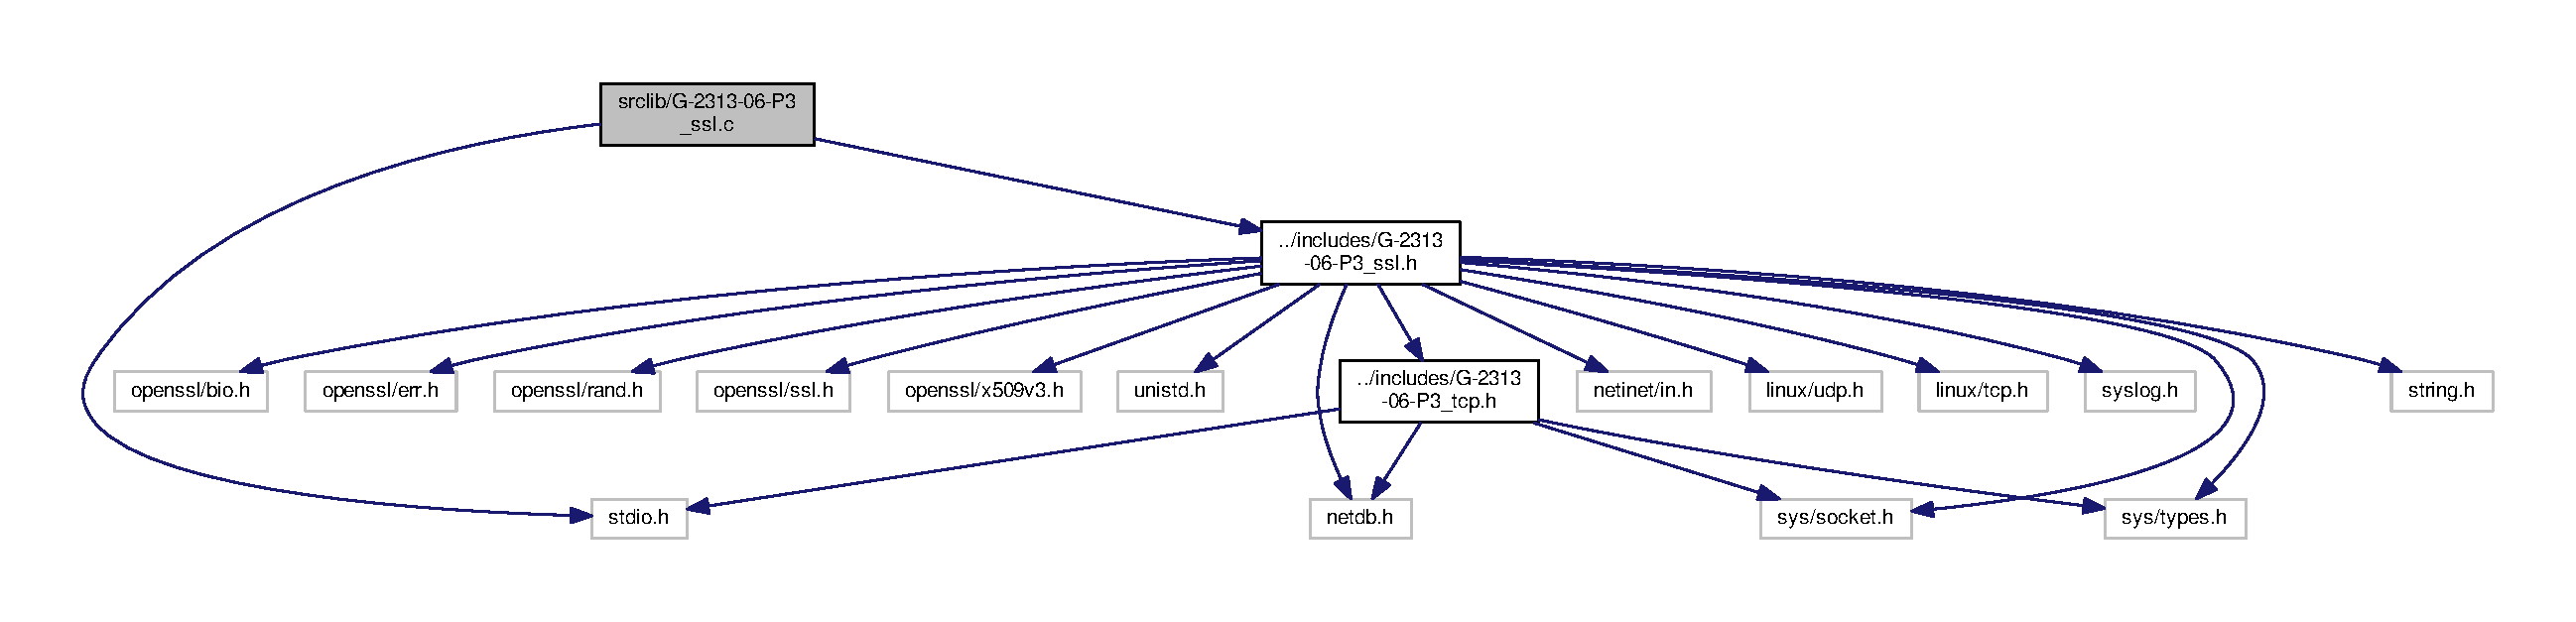
\includegraphics[width=350pt]{G-2313-06-P3__ssl_8c__incl}
\end{center}
\end{figure}
\subsection*{Funciones}
\begin{DoxyCompactItemize}
\item 
void \hyperlink{G-2313-06-P3__ssl_8c_a0fc205ff57c9c0a489d8154f94cd2f4a}{ssl\+\_\+start\+\_\+client} ()
\item 
void \hyperlink{G-2313-06-P3__ssl_8c_a6dcf2890813db3e4f8f2f423716d4883}{ssl\+\_\+start\+\_\+server} ()
\item 
S\+S\+L\+\_\+\+C\+TX $\ast$ \hyperlink{G-2313-06-P3__ssl_8c_a32d6d68d1f64d25effa1ea5ec1e6bdb3}{inicializar\+\_\+nivel\+\_\+\+S\+SL} (int $\ast$desc)
\item 
int \hyperlink{G-2313-06-P3__ssl_8c_a44410967ff9e0a1b4219c85f0e62e926}{aceptar\+\_\+canal\+\_\+seguro\+\_\+\+S\+SL} (S\+S\+L\+\_\+\+C\+TX $\ast$ctx\+\_\+ssl, S\+SL $\ast$$\ast$ssl, int desc, int puerto, int tam, struct sockaddr\+\_\+in ip4addr)
\item 
int \hyperlink{G-2313-06-P3__ssl_8c_ac5f32cf09e3c0efd5cbc25452ed192a9}{evaluar\+\_\+post\+\_\+connectar\+\_\+\+S\+SL} (S\+SL $\ast$ssl)
\item 
int \hyperlink{G-2313-06-P3__ssl_8c_adf9cb4f6b9c27081fcf12a942db1b288}{enviar\+\_\+datos\+\_\+\+S\+SL} (S\+SL $\ast$ssl, const char $\ast$buf)
\item 
int \hyperlink{G-2313-06-P3__ssl_8c_af7dca116c6dbb68e9609293102c208c5}{recibir\+\_\+datos\+\_\+\+S\+SL} (S\+SL $\ast$ssl, char $\ast$buf)
\item 
int \hyperlink{G-2313-06-P3__ssl_8c_a006acb44fc7dae799271a48117f5a398}{fijar\+\_\+contexto\+\_\+\+S\+SL} (S\+S\+L\+\_\+\+C\+TX $\ast$ssl\+\_\+ctx, char $\ast$cert\+File, char $\ast$cert\+Root)
\item 
void \hyperlink{G-2313-06-P3__ssl_8c_a307ee105b4b24b555d8df68603c2deff}{cerrar\+\_\+canal\+\_\+\+S\+SL} (S\+SL $\ast$ssl, S\+S\+L\+\_\+\+C\+TX $\ast$ctl\+\_\+ssl, int desc)
\item 
S\+SL $\ast$ \hyperlink{G-2313-06-P3__ssl_8c_aa58ddc931cb106d430ab49223b9394fc}{conectar\+\_\+canal\+\_\+seguro\+\_\+\+S\+SL} (S\+S\+L\+\_\+\+C\+TX $\ast$ctx\+\_\+ssl, int desc, struct sockaddr res)
\end{DoxyCompactItemize}


\subsection{Documentación de las funciones}
\index{G-\/2313-\/06-\/\+P3\+\_\+ssl.\+c@{G-\/2313-\/06-\/\+P3\+\_\+ssl.\+c}!aceptar\+\_\+canal\+\_\+seguro\+\_\+\+S\+SL@{aceptar\+\_\+canal\+\_\+seguro\+\_\+\+S\+SL}}
\index{aceptar\+\_\+canal\+\_\+seguro\+\_\+\+S\+SL@{aceptar\+\_\+canal\+\_\+seguro\+\_\+\+S\+SL}!G-\/2313-\/06-\/\+P3\+\_\+ssl.\+c@{G-\/2313-\/06-\/\+P3\+\_\+ssl.\+c}}
\subsubsection[{\texorpdfstring{aceptar\+\_\+canal\+\_\+seguro\+\_\+\+S\+S\+L(\+S\+S\+L\+\_\+\+C\+T\+X $\ast$ctx\+\_\+ssl, S\+S\+L $\ast$$\ast$ssl, int desc, int puerto, int tam, struct sockaddr\+\_\+in ip4addr)}{aceptar_canal_seguro_SSL(SSL_CTX *ctx_ssl, SSL **ssl, int desc, int puerto, int tam, struct sockaddr_in ip4addr)}}]{\setlength{\rightskip}{0pt plus 5cm}int aceptar\+\_\+canal\+\_\+seguro\+\_\+\+S\+SL (
\begin{DoxyParamCaption}
\item[{S\+S\+L\+\_\+\+C\+TX $\ast$}]{ctx\+\_\+ssl, }
\item[{S\+SL $\ast$$\ast$}]{ssl, }
\item[{int}]{desc, }
\item[{int}]{puerto, }
\item[{int}]{tam, }
\item[{struct sockaddr\+\_\+in}]{ip4addr}
\end{DoxyParamCaption}
)}\hypertarget{G-2313-06-P3__ssl_8c_a44410967ff9e0a1b4219c85f0e62e926}{}\label{G-2313-06-P3__ssl_8c_a44410967ff9e0a1b4219c85f0e62e926}


Definición en la línea 231 del archivo G-\/2313-\/06-\/\+P3\+\_\+ssl.\+c.

\index{G-\/2313-\/06-\/\+P3\+\_\+ssl.\+c@{G-\/2313-\/06-\/\+P3\+\_\+ssl.\+c}!cerrar\+\_\+canal\+\_\+\+S\+SL@{cerrar\+\_\+canal\+\_\+\+S\+SL}}
\index{cerrar\+\_\+canal\+\_\+\+S\+SL@{cerrar\+\_\+canal\+\_\+\+S\+SL}!G-\/2313-\/06-\/\+P3\+\_\+ssl.\+c@{G-\/2313-\/06-\/\+P3\+\_\+ssl.\+c}}
\subsubsection[{\texorpdfstring{cerrar\+\_\+canal\+\_\+\+S\+S\+L(\+S\+S\+L $\ast$ssl, S\+S\+L\+\_\+\+C\+T\+X $\ast$ctl\+\_\+ssl, int desc)}{cerrar_canal_SSL(SSL *ssl, SSL_CTX *ctl_ssl, int desc)}}]{\setlength{\rightskip}{0pt plus 5cm}void cerrar\+\_\+canal\+\_\+\+S\+SL (
\begin{DoxyParamCaption}
\item[{S\+SL $\ast$}]{ssl, }
\item[{S\+S\+L\+\_\+\+C\+TX $\ast$}]{ctl\+\_\+ssl, }
\item[{int}]{desc}
\end{DoxyParamCaption}
)}\hypertarget{G-2313-06-P3__ssl_8c_a307ee105b4b24b555d8df68603c2deff}{}\label{G-2313-06-P3__ssl_8c_a307ee105b4b24b555d8df68603c2deff}


Definición en la línea 441 del archivo G-\/2313-\/06-\/\+P3\+\_\+ssl.\+c.

\index{G-\/2313-\/06-\/\+P3\+\_\+ssl.\+c@{G-\/2313-\/06-\/\+P3\+\_\+ssl.\+c}!conectar\+\_\+canal\+\_\+seguro\+\_\+\+S\+SL@{conectar\+\_\+canal\+\_\+seguro\+\_\+\+S\+SL}}
\index{conectar\+\_\+canal\+\_\+seguro\+\_\+\+S\+SL@{conectar\+\_\+canal\+\_\+seguro\+\_\+\+S\+SL}!G-\/2313-\/06-\/\+P3\+\_\+ssl.\+c@{G-\/2313-\/06-\/\+P3\+\_\+ssl.\+c}}
\subsubsection[{\texorpdfstring{conectar\+\_\+canal\+\_\+seguro\+\_\+\+S\+S\+L(\+S\+S\+L\+\_\+\+C\+T\+X $\ast$ctx\+\_\+ssl, int desc, struct sockaddr res)}{conectar_canal_seguro_SSL(SSL_CTX *ctx_ssl, int desc, struct sockaddr res)}}]{\setlength{\rightskip}{0pt plus 5cm}S\+SL$\ast$ conectar\+\_\+canal\+\_\+seguro\+\_\+\+S\+SL (
\begin{DoxyParamCaption}
\item[{S\+S\+L\+\_\+\+C\+TX $\ast$}]{ctx\+\_\+ssl, }
\item[{int}]{desc, }
\item[{struct sockaddr}]{res}
\end{DoxyParamCaption}
)}\hypertarget{G-2313-06-P3__ssl_8c_aa58ddc931cb106d430ab49223b9394fc}{}\label{G-2313-06-P3__ssl_8c_aa58ddc931cb106d430ab49223b9394fc}


Definición en la línea 484 del archivo G-\/2313-\/06-\/\+P3\+\_\+ssl.\+c.

\index{G-\/2313-\/06-\/\+P3\+\_\+ssl.\+c@{G-\/2313-\/06-\/\+P3\+\_\+ssl.\+c}!enviar\+\_\+datos\+\_\+\+S\+SL@{enviar\+\_\+datos\+\_\+\+S\+SL}}
\index{enviar\+\_\+datos\+\_\+\+S\+SL@{enviar\+\_\+datos\+\_\+\+S\+SL}!G-\/2313-\/06-\/\+P3\+\_\+ssl.\+c@{G-\/2313-\/06-\/\+P3\+\_\+ssl.\+c}}
\subsubsection[{\texorpdfstring{enviar\+\_\+datos\+\_\+\+S\+S\+L(\+S\+S\+L $\ast$ssl, const char $\ast$buf)}{enviar_datos_SSL(SSL *ssl, const char *buf)}}]{\setlength{\rightskip}{0pt plus 5cm}int enviar\+\_\+datos\+\_\+\+S\+SL (
\begin{DoxyParamCaption}
\item[{S\+SL $\ast$}]{ssl, }
\item[{const char $\ast$}]{buf}
\end{DoxyParamCaption}
)}\hypertarget{G-2313-06-P3__ssl_8c_adf9cb4f6b9c27081fcf12a942db1b288}{}\label{G-2313-06-P3__ssl_8c_adf9cb4f6b9c27081fcf12a942db1b288}


Definición en la línea 322 del archivo G-\/2313-\/06-\/\+P3\+\_\+ssl.\+c.

\index{G-\/2313-\/06-\/\+P3\+\_\+ssl.\+c@{G-\/2313-\/06-\/\+P3\+\_\+ssl.\+c}!evaluar\+\_\+post\+\_\+connectar\+\_\+\+S\+SL@{evaluar\+\_\+post\+\_\+connectar\+\_\+\+S\+SL}}
\index{evaluar\+\_\+post\+\_\+connectar\+\_\+\+S\+SL@{evaluar\+\_\+post\+\_\+connectar\+\_\+\+S\+SL}!G-\/2313-\/06-\/\+P3\+\_\+ssl.\+c@{G-\/2313-\/06-\/\+P3\+\_\+ssl.\+c}}
\subsubsection[{\texorpdfstring{evaluar\+\_\+post\+\_\+connectar\+\_\+\+S\+S\+L(\+S\+S\+L $\ast$ssl)}{evaluar_post_connectar_SSL(SSL *ssl)}}]{\setlength{\rightskip}{0pt plus 5cm}int evaluar\+\_\+post\+\_\+connectar\+\_\+\+S\+SL (
\begin{DoxyParamCaption}
\item[{S\+SL $\ast$}]{ssl}
\end{DoxyParamCaption}
)}\hypertarget{G-2313-06-P3__ssl_8c_ac5f32cf09e3c0efd5cbc25452ed192a9}{}\label{G-2313-06-P3__ssl_8c_ac5f32cf09e3c0efd5cbc25452ed192a9}


Definición en la línea 284 del archivo G-\/2313-\/06-\/\+P3\+\_\+ssl.\+c.

\index{G-\/2313-\/06-\/\+P3\+\_\+ssl.\+c@{G-\/2313-\/06-\/\+P3\+\_\+ssl.\+c}!fijar\+\_\+contexto\+\_\+\+S\+SL@{fijar\+\_\+contexto\+\_\+\+S\+SL}}
\index{fijar\+\_\+contexto\+\_\+\+S\+SL@{fijar\+\_\+contexto\+\_\+\+S\+SL}!G-\/2313-\/06-\/\+P3\+\_\+ssl.\+c@{G-\/2313-\/06-\/\+P3\+\_\+ssl.\+c}}
\subsubsection[{\texorpdfstring{fijar\+\_\+contexto\+\_\+\+S\+S\+L(\+S\+S\+L\+\_\+\+C\+T\+X $\ast$ssl\+\_\+ctx, char $\ast$cert\+File, char $\ast$cert\+Root)}{fijar_contexto_SSL(SSL_CTX *ssl_ctx, char *certFile, char *certRoot)}}]{\setlength{\rightskip}{0pt plus 5cm}int fijar\+\_\+contexto\+\_\+\+S\+SL (
\begin{DoxyParamCaption}
\item[{S\+S\+L\+\_\+\+C\+TX $\ast$}]{ssl\+\_\+ctx, }
\item[{char $\ast$}]{cert\+File, }
\item[{char $\ast$}]{cert\+Root}
\end{DoxyParamCaption}
)}\hypertarget{G-2313-06-P3__ssl_8c_a006acb44fc7dae799271a48117f5a398}{}\label{G-2313-06-P3__ssl_8c_a006acb44fc7dae799271a48117f5a398}


Definición en la línea 392 del archivo G-\/2313-\/06-\/\+P3\+\_\+ssl.\+c.

\index{G-\/2313-\/06-\/\+P3\+\_\+ssl.\+c@{G-\/2313-\/06-\/\+P3\+\_\+ssl.\+c}!inicializar\+\_\+nivel\+\_\+\+S\+SL@{inicializar\+\_\+nivel\+\_\+\+S\+SL}}
\index{inicializar\+\_\+nivel\+\_\+\+S\+SL@{inicializar\+\_\+nivel\+\_\+\+S\+SL}!G-\/2313-\/06-\/\+P3\+\_\+ssl.\+c@{G-\/2313-\/06-\/\+P3\+\_\+ssl.\+c}}
\subsubsection[{\texorpdfstring{inicializar\+\_\+nivel\+\_\+\+S\+S\+L(int $\ast$desc)}{inicializar_nivel_SSL(int *desc)}}]{\setlength{\rightskip}{0pt plus 5cm}S\+S\+L\+\_\+\+C\+TX$\ast$ inicializar\+\_\+nivel\+\_\+\+S\+SL (
\begin{DoxyParamCaption}
\item[{int $\ast$}]{desc}
\end{DoxyParamCaption}
)}\hypertarget{G-2313-06-P3__ssl_8c_a32d6d68d1f64d25effa1ea5ec1e6bdb3}{}\label{G-2313-06-P3__ssl_8c_a32d6d68d1f64d25effa1ea5ec1e6bdb3}


Definición en la línea 183 del archivo G-\/2313-\/06-\/\+P3\+\_\+ssl.\+c.

\index{G-\/2313-\/06-\/\+P3\+\_\+ssl.\+c@{G-\/2313-\/06-\/\+P3\+\_\+ssl.\+c}!recibir\+\_\+datos\+\_\+\+S\+SL@{recibir\+\_\+datos\+\_\+\+S\+SL}}
\index{recibir\+\_\+datos\+\_\+\+S\+SL@{recibir\+\_\+datos\+\_\+\+S\+SL}!G-\/2313-\/06-\/\+P3\+\_\+ssl.\+c@{G-\/2313-\/06-\/\+P3\+\_\+ssl.\+c}}
\subsubsection[{\texorpdfstring{recibir\+\_\+datos\+\_\+\+S\+S\+L(\+S\+S\+L $\ast$ssl, char $\ast$buf)}{recibir_datos_SSL(SSL *ssl, char *buf)}}]{\setlength{\rightskip}{0pt plus 5cm}int recibir\+\_\+datos\+\_\+\+S\+SL (
\begin{DoxyParamCaption}
\item[{S\+SL $\ast$}]{ssl, }
\item[{char $\ast$}]{buf}
\end{DoxyParamCaption}
)}\hypertarget{G-2313-06-P3__ssl_8c_af7dca116c6dbb68e9609293102c208c5}{}\label{G-2313-06-P3__ssl_8c_af7dca116c6dbb68e9609293102c208c5}


Definición en la línea 354 del archivo G-\/2313-\/06-\/\+P3\+\_\+ssl.\+c.

\index{G-\/2313-\/06-\/\+P3\+\_\+ssl.\+c@{G-\/2313-\/06-\/\+P3\+\_\+ssl.\+c}!ssl\+\_\+start\+\_\+client@{ssl\+\_\+start\+\_\+client}}
\index{ssl\+\_\+start\+\_\+client@{ssl\+\_\+start\+\_\+client}!G-\/2313-\/06-\/\+P3\+\_\+ssl.\+c@{G-\/2313-\/06-\/\+P3\+\_\+ssl.\+c}}
\subsubsection[{\texorpdfstring{ssl\+\_\+start\+\_\+client()}{ssl_start_client()}}]{\setlength{\rightskip}{0pt plus 5cm}void ssl\+\_\+start\+\_\+client (
\begin{DoxyParamCaption}
{}
\end{DoxyParamCaption}
)}\hypertarget{G-2313-06-P3__ssl_8c_a0fc205ff57c9c0a489d8154f94cd2f4a}{}\label{G-2313-06-P3__ssl_8c_a0fc205ff57c9c0a489d8154f94cd2f4a}


Definición en la línea 26 del archivo G-\/2313-\/06-\/\+P3\+\_\+ssl.\+c.

\index{G-\/2313-\/06-\/\+P3\+\_\+ssl.\+c@{G-\/2313-\/06-\/\+P3\+\_\+ssl.\+c}!ssl\+\_\+start\+\_\+server@{ssl\+\_\+start\+\_\+server}}
\index{ssl\+\_\+start\+\_\+server@{ssl\+\_\+start\+\_\+server}!G-\/2313-\/06-\/\+P3\+\_\+ssl.\+c@{G-\/2313-\/06-\/\+P3\+\_\+ssl.\+c}}
\subsubsection[{\texorpdfstring{ssl\+\_\+start\+\_\+server()}{ssl_start_server()}}]{\setlength{\rightskip}{0pt plus 5cm}void ssl\+\_\+start\+\_\+server (
\begin{DoxyParamCaption}
{}
\end{DoxyParamCaption}
)}\hypertarget{G-2313-06-P3__ssl_8c_a6dcf2890813db3e4f8f2f423716d4883}{}\label{G-2313-06-P3__ssl_8c_a6dcf2890813db3e4f8f2f423716d4883}


Definición en la línea 95 del archivo G-\/2313-\/06-\/\+P3\+\_\+ssl.\+c.


\hypertarget{G-2313-06-P3__tcp_8c}{}\section{Referencia del Archivo srclib/\+G-\/2313-\/06-\/\+P3\+\_\+tcp.c}
\label{G-2313-06-P3__tcp_8c}\index{srclib/\+G-\/2313-\/06-\/\+P3\+\_\+tcp.\+c@{srclib/\+G-\/2313-\/06-\/\+P3\+\_\+tcp.\+c}}
{\ttfamily \#include \char`\"{}../includes/\+G-\/2313-\/06-\/\+P3\+\_\+tcp.\+h\char`\"{}}\\*
{\ttfamily \#include $<$sys/socket.\+h$>$}\\*
{\ttfamily \#include $<$string.\+h$>$}\\*
{\ttfamily \#include $<$netdb.\+h$>$}\\*
{\ttfamily \#include $<$unistd.\+h$>$}\\*
Dependencia gráfica adjunta para G-\/2313-\/06-\/\+P3\+\_\+tcp.c\+:
\nopagebreak
\begin{figure}[H]
\begin{center}
\leavevmode
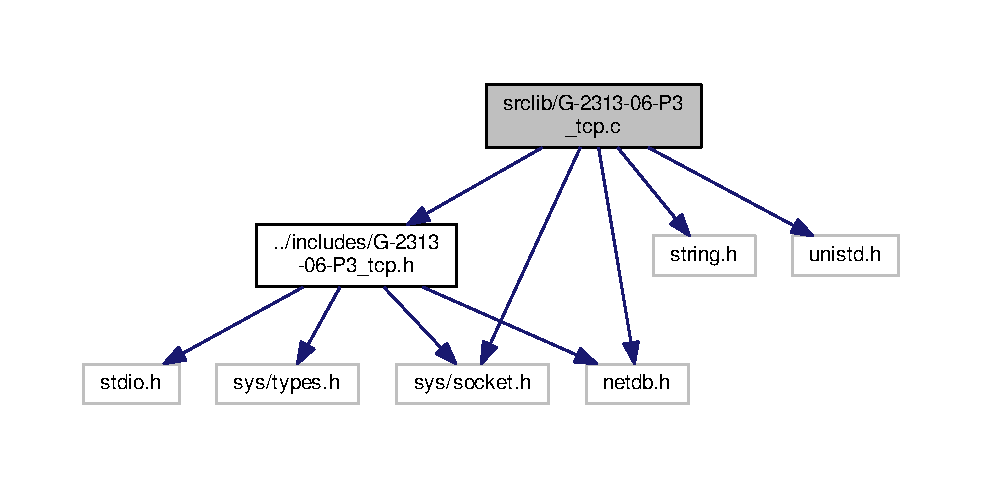
\includegraphics[width=350pt]{G-2313-06-P3__tcp_8c__incl}
\end{center}
\end{figure}
\subsection*{Funciones}
\begin{DoxyCompactItemize}
\item 
int \hyperlink{G-2313-06-P3__tcp_8c_a25c77773298f02f1e8135829713d7f3a}{tcp\+\_\+new\+\_\+socket} ()
\item 
int \hyperlink{G-2313-06-P3__tcp_8c_a383b8c763aedca0e2ed838e32073fde6}{tcp\+\_\+bind} (int desc, int puerto)
\item 
int \hyperlink{G-2313-06-P3__tcp_8c_a9c9d03de1e87014ced69f8d36bb37f86}{tcp\+\_\+new\+\_\+listen} (int desc, int tam)
\item 
int \hyperlink{G-2313-06-P3__tcp_8c_a6bae59be22b410f157347083f2e43987}{tcp\+\_\+new\+\_\+accept} (int desc, struct sockaddr\+\_\+in ip4addr)
\item 
int \hyperlink{G-2313-06-P3__tcp_8c_a3e15d12d1405c959da073cabab3a8520}{tcp\+\_\+new\+\_\+open\+\_\+connection} (int desc, struct sockaddr res)
\item 
int \hyperlink{G-2313-06-P3__tcp_8c_a4e5ce422aa030ac8b3998e858b79cae2}{tcp\+\_\+connect} (char $\ast$server, int port)
\item 
int \hyperlink{G-2313-06-P3__tcp_8c_a14d727cfbcd2ce3c5f4fae5a470a84da}{tcp\+\_\+listen} (int port, int max\+\_\+conn)
\item 
int \hyperlink{G-2313-06-P3__tcp_8c_a1e2b75e457a02f23d433a6821f6902b7}{tcp\+\_\+send} (int fd, char $\ast$msg)
\item 
int \hyperlink{G-2313-06-P3__tcp_8c_af3354e60e1181adcd72f9f242063fafe}{tcp\+\_\+receive} (int fd, char $\ast$msg, int len)
\item 
int \hyperlink{G-2313-06-P3__tcp_8c_a2d1f9e76e5da3a7c1e172d1294a33611}{tcp\+\_\+disconnect} (int fd)
\end{DoxyCompactItemize}


\subsection{Documentación de las funciones}
\index{G-\/2313-\/06-\/\+P3\+\_\+tcp.\+c@{G-\/2313-\/06-\/\+P3\+\_\+tcp.\+c}!tcp\+\_\+bind@{tcp\+\_\+bind}}
\index{tcp\+\_\+bind@{tcp\+\_\+bind}!G-\/2313-\/06-\/\+P3\+\_\+tcp.\+c@{G-\/2313-\/06-\/\+P3\+\_\+tcp.\+c}}
\subsubsection[{\texorpdfstring{tcp\+\_\+bind(int desc, int puerto)}{tcp_bind(int desc, int puerto)}}]{\setlength{\rightskip}{0pt plus 5cm}int tcp\+\_\+bind (
\begin{DoxyParamCaption}
\item[{int}]{desc, }
\item[{int}]{puerto}
\end{DoxyParamCaption}
)}\hypertarget{G-2313-06-P3__tcp_8c_a383b8c763aedca0e2ed838e32073fde6}{}\label{G-2313-06-P3__tcp_8c_a383b8c763aedca0e2ed838e32073fde6}


Definición en la línea 14 del archivo G-\/2313-\/06-\/\+P3\+\_\+tcp.\+c.

\index{G-\/2313-\/06-\/\+P3\+\_\+tcp.\+c@{G-\/2313-\/06-\/\+P3\+\_\+tcp.\+c}!tcp\+\_\+connect@{tcp\+\_\+connect}}
\index{tcp\+\_\+connect@{tcp\+\_\+connect}!G-\/2313-\/06-\/\+P3\+\_\+tcp.\+c@{G-\/2313-\/06-\/\+P3\+\_\+tcp.\+c}}
\subsubsection[{\texorpdfstring{tcp\+\_\+connect(char $\ast$server, int port)}{tcp_connect(char *server, int port)}}]{\setlength{\rightskip}{0pt plus 5cm}int tcp\+\_\+connect (
\begin{DoxyParamCaption}
\item[{char $\ast$}]{server, }
\item[{int}]{port}
\end{DoxyParamCaption}
)}\hypertarget{G-2313-06-P3__tcp_8c_a4e5ce422aa030ac8b3998e858b79cae2}{}\label{G-2313-06-P3__tcp_8c_a4e5ce422aa030ac8b3998e858b79cae2}


Definición en la línea 51 del archivo G-\/2313-\/06-\/\+P3\+\_\+tcp.\+c.

\index{G-\/2313-\/06-\/\+P3\+\_\+tcp.\+c@{G-\/2313-\/06-\/\+P3\+\_\+tcp.\+c}!tcp\+\_\+disconnect@{tcp\+\_\+disconnect}}
\index{tcp\+\_\+disconnect@{tcp\+\_\+disconnect}!G-\/2313-\/06-\/\+P3\+\_\+tcp.\+c@{G-\/2313-\/06-\/\+P3\+\_\+tcp.\+c}}
\subsubsection[{\texorpdfstring{tcp\+\_\+disconnect(int fd)}{tcp_disconnect(int fd)}}]{\setlength{\rightskip}{0pt plus 5cm}int tcp\+\_\+disconnect (
\begin{DoxyParamCaption}
\item[{int}]{fd}
\end{DoxyParamCaption}
)}\hypertarget{G-2313-06-P3__tcp_8c_a2d1f9e76e5da3a7c1e172d1294a33611}{}\label{G-2313-06-P3__tcp_8c_a2d1f9e76e5da3a7c1e172d1294a33611}


Definición en la línea 132 del archivo G-\/2313-\/06-\/\+P3\+\_\+tcp.\+c.

\index{G-\/2313-\/06-\/\+P3\+\_\+tcp.\+c@{G-\/2313-\/06-\/\+P3\+\_\+tcp.\+c}!tcp\+\_\+listen@{tcp\+\_\+listen}}
\index{tcp\+\_\+listen@{tcp\+\_\+listen}!G-\/2313-\/06-\/\+P3\+\_\+tcp.\+c@{G-\/2313-\/06-\/\+P3\+\_\+tcp.\+c}}
\subsubsection[{\texorpdfstring{tcp\+\_\+listen(int port, int max\+\_\+conn)}{tcp_listen(int port, int max_conn)}}]{\setlength{\rightskip}{0pt plus 5cm}int tcp\+\_\+listen (
\begin{DoxyParamCaption}
\item[{int}]{port, }
\item[{int}]{max\+\_\+conn}
\end{DoxyParamCaption}
)}\hypertarget{G-2313-06-P3__tcp_8c_a14d727cfbcd2ce3c5f4fae5a470a84da}{}\label{G-2313-06-P3__tcp_8c_a14d727cfbcd2ce3c5f4fae5a470a84da}


Definición en la línea 83 del archivo G-\/2313-\/06-\/\+P3\+\_\+tcp.\+c.

\index{G-\/2313-\/06-\/\+P3\+\_\+tcp.\+c@{G-\/2313-\/06-\/\+P3\+\_\+tcp.\+c}!tcp\+\_\+new\+\_\+accept@{tcp\+\_\+new\+\_\+accept}}
\index{tcp\+\_\+new\+\_\+accept@{tcp\+\_\+new\+\_\+accept}!G-\/2313-\/06-\/\+P3\+\_\+tcp.\+c@{G-\/2313-\/06-\/\+P3\+\_\+tcp.\+c}}
\subsubsection[{\texorpdfstring{tcp\+\_\+new\+\_\+accept(int desc, struct sockaddr\+\_\+in ip4addr)}{tcp_new_accept(int desc, struct sockaddr_in ip4addr)}}]{\setlength{\rightskip}{0pt plus 5cm}int tcp\+\_\+new\+\_\+accept (
\begin{DoxyParamCaption}
\item[{int}]{desc, }
\item[{struct sockaddr\+\_\+in}]{ip4addr}
\end{DoxyParamCaption}
)}\hypertarget{G-2313-06-P3__tcp_8c_a6bae59be22b410f157347083f2e43987}{}\label{G-2313-06-P3__tcp_8c_a6bae59be22b410f157347083f2e43987}


Definición en la línea 33 del archivo G-\/2313-\/06-\/\+P3\+\_\+tcp.\+c.

\index{G-\/2313-\/06-\/\+P3\+\_\+tcp.\+c@{G-\/2313-\/06-\/\+P3\+\_\+tcp.\+c}!tcp\+\_\+new\+\_\+listen@{tcp\+\_\+new\+\_\+listen}}
\index{tcp\+\_\+new\+\_\+listen@{tcp\+\_\+new\+\_\+listen}!G-\/2313-\/06-\/\+P3\+\_\+tcp.\+c@{G-\/2313-\/06-\/\+P3\+\_\+tcp.\+c}}
\subsubsection[{\texorpdfstring{tcp\+\_\+new\+\_\+listen(int desc, int tam)}{tcp_new_listen(int desc, int tam)}}]{\setlength{\rightskip}{0pt plus 5cm}int tcp\+\_\+new\+\_\+listen (
\begin{DoxyParamCaption}
\item[{int}]{desc, }
\item[{int}]{tam}
\end{DoxyParamCaption}
)}\hypertarget{G-2313-06-P3__tcp_8c_a9c9d03de1e87014ced69f8d36bb37f86}{}\label{G-2313-06-P3__tcp_8c_a9c9d03de1e87014ced69f8d36bb37f86}


Definición en la línea 25 del archivo G-\/2313-\/06-\/\+P3\+\_\+tcp.\+c.

\index{G-\/2313-\/06-\/\+P3\+\_\+tcp.\+c@{G-\/2313-\/06-\/\+P3\+\_\+tcp.\+c}!tcp\+\_\+new\+\_\+open\+\_\+connection@{tcp\+\_\+new\+\_\+open\+\_\+connection}}
\index{tcp\+\_\+new\+\_\+open\+\_\+connection@{tcp\+\_\+new\+\_\+open\+\_\+connection}!G-\/2313-\/06-\/\+P3\+\_\+tcp.\+c@{G-\/2313-\/06-\/\+P3\+\_\+tcp.\+c}}
\subsubsection[{\texorpdfstring{tcp\+\_\+new\+\_\+open\+\_\+connection(int desc, struct sockaddr res)}{tcp_new_open_connection(int desc, struct sockaddr res)}}]{\setlength{\rightskip}{0pt plus 5cm}int tcp\+\_\+new\+\_\+open\+\_\+connection (
\begin{DoxyParamCaption}
\item[{int}]{desc, }
\item[{struct sockaddr}]{res}
\end{DoxyParamCaption}
)}\hypertarget{G-2313-06-P3__tcp_8c_a3e15d12d1405c959da073cabab3a8520}{}\label{G-2313-06-P3__tcp_8c_a3e15d12d1405c959da073cabab3a8520}


Definición en la línea 43 del archivo G-\/2313-\/06-\/\+P3\+\_\+tcp.\+c.

\index{G-\/2313-\/06-\/\+P3\+\_\+tcp.\+c@{G-\/2313-\/06-\/\+P3\+\_\+tcp.\+c}!tcp\+\_\+new\+\_\+socket@{tcp\+\_\+new\+\_\+socket}}
\index{tcp\+\_\+new\+\_\+socket@{tcp\+\_\+new\+\_\+socket}!G-\/2313-\/06-\/\+P3\+\_\+tcp.\+c@{G-\/2313-\/06-\/\+P3\+\_\+tcp.\+c}}
\subsubsection[{\texorpdfstring{tcp\+\_\+new\+\_\+socket()}{tcp_new_socket()}}]{\setlength{\rightskip}{0pt plus 5cm}int tcp\+\_\+new\+\_\+socket (
\begin{DoxyParamCaption}
{}
\end{DoxyParamCaption}
)}\hypertarget{G-2313-06-P3__tcp_8c_a25c77773298f02f1e8135829713d7f3a}{}\label{G-2313-06-P3__tcp_8c_a25c77773298f02f1e8135829713d7f3a}


Definición en la línea 7 del archivo G-\/2313-\/06-\/\+P3\+\_\+tcp.\+c.

\index{G-\/2313-\/06-\/\+P3\+\_\+tcp.\+c@{G-\/2313-\/06-\/\+P3\+\_\+tcp.\+c}!tcp\+\_\+receive@{tcp\+\_\+receive}}
\index{tcp\+\_\+receive@{tcp\+\_\+receive}!G-\/2313-\/06-\/\+P3\+\_\+tcp.\+c@{G-\/2313-\/06-\/\+P3\+\_\+tcp.\+c}}
\subsubsection[{\texorpdfstring{tcp\+\_\+receive(int fd, char $\ast$msg, int len)}{tcp_receive(int fd, char *msg, int len)}}]{\setlength{\rightskip}{0pt plus 5cm}int tcp\+\_\+receive (
\begin{DoxyParamCaption}
\item[{int}]{fd, }
\item[{char $\ast$}]{msg, }
\item[{int}]{len}
\end{DoxyParamCaption}
)}\hypertarget{G-2313-06-P3__tcp_8c_af3354e60e1181adcd72f9f242063fafe}{}\label{G-2313-06-P3__tcp_8c_af3354e60e1181adcd72f9f242063fafe}


Definición en la línea 125 del archivo G-\/2313-\/06-\/\+P3\+\_\+tcp.\+c.

\index{G-\/2313-\/06-\/\+P3\+\_\+tcp.\+c@{G-\/2313-\/06-\/\+P3\+\_\+tcp.\+c}!tcp\+\_\+send@{tcp\+\_\+send}}
\index{tcp\+\_\+send@{tcp\+\_\+send}!G-\/2313-\/06-\/\+P3\+\_\+tcp.\+c@{G-\/2313-\/06-\/\+P3\+\_\+tcp.\+c}}
\subsubsection[{\texorpdfstring{tcp\+\_\+send(int fd, char $\ast$msg)}{tcp_send(int fd, char *msg)}}]{\setlength{\rightskip}{0pt plus 5cm}int tcp\+\_\+send (
\begin{DoxyParamCaption}
\item[{int}]{fd, }
\item[{char $\ast$}]{msg}
\end{DoxyParamCaption}
)}\hypertarget{G-2313-06-P3__tcp_8c_a1e2b75e457a02f23d433a6821f6902b7}{}\label{G-2313-06-P3__tcp_8c_a1e2b75e457a02f23d433a6821f6902b7}


Definición en la línea 118 del archivo G-\/2313-\/06-\/\+P3\+\_\+tcp.\+c.


%--- End generated contents ---

% Index
\backmatter
\newpage
\phantomsection
\clearemptydoublepage
\addcontentsline{toc}{chapter}{Índice}
\printindex

\end{document}
